%% LyX 2.3.7 created this file.  For more info, see http://www.lyx.org/.
%% Do not edit unless you really know what you are doing.
\documentclass[12pt,hyperfootnotes=false]{article}
\usepackage{mathptmx}
\usepackage[latin9]{inputenc}
\usepackage{geometry}
\geometry{verbose,tmargin=1in,bmargin=1in,lmargin=1in,rmargin=1in}
\usepackage{float}
\usepackage{amsmath}
\usepackage{amsthm}
\usepackage{amssymb}
\usepackage{graphicx}
\usepackage{setspace}
\usepackage[authoryear]{natbib}
\onehalfspacing

\makeatletter

%%%%%%%%%%%%%%%%%%%%%%%%%%%%%% LyX specific LaTeX commands.
%% Because html converters don't know tabularnewline
\providecommand{\tabularnewline}{\\}

%%%%%%%%%%%%%%%%%%%%%%%%%%%%%% User specified LaTeX commands.
\usepackage{amsthm}
\usepackage{bm}
\usepackage{setspace}
\usepackage{sectsty}

\usepackage{datetime}
\usepackage{pdflscape}
\usepackage[english]{babel}
\usepackage{times}
\usepackage[small]{caption}
\usepackage[bottom,hang,flushmargin]{footmisc}

\DeclareMathOperator{\sgn}{sgn}
\DeclareMathOperator{\Var}{Var}
\DeclareMathOperator{\Corr}{Corr}
\DeclareMathOperator{\Cov}{Cov}
\DeclareMathOperator{\E}{E}
\DeclareMathOperator{\logit}{logit}
\DeclareMathOperator{\I}{I}

\sectionfont{\noindent\normalfont\large\bf}
\subsectionfont{\noindent\normalfont\normalsize\bf}
\subsubsectionfont{\noindent\normalfont\it}

\pdfminorversion=4

\makeatother

\begin{document}
\title{\noindent \textbf{Title}}
\author{\noindent Author 1,\textbf{ }\textit{Affiliation 1}\textbf{}\thanks{E-mail:\ author1@affiliation1.edu, author2@affiliation2.edu. Acknowledgements
here.}\textbf{}\\
Author 2, \textit{Affiliation 2}\textbf{}\\
}
\date{\monthname\ \number\year}
\maketitle
\begin{abstract}
\noindent The abstract.

\bigskip{}
\end{abstract}
\pagebreak{}

\begin{spacing}{1.4}

\section{Introduction}

\end{spacing}

\pagebreak{}

\section*{References}

\leftskip=2em 
\parindent=-2em
\onehalfspacing

\noindent

Last, First. Year. Title. \textit{Journal} Volume\#(issue\#): page
range.

\parindent=2em
\leftskip=0em

\pagebreak{}

\begin{figure}[H]
\caption{Figure Title}

\begin{centering}
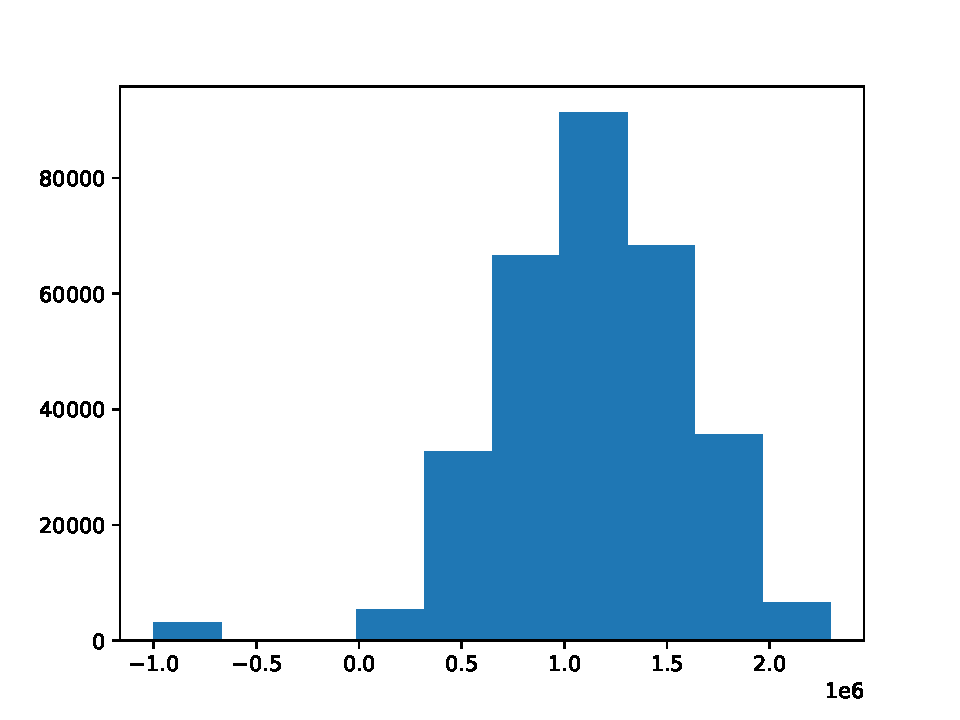
\includegraphics[scale=0.7]{../input/chips_sold}
\par\end{centering}
Note: Figure note
\end{figure}



\clearpage

\noindent 
\begin{table}[H]
\caption{Table Title\label{tab:regression}}
\medskip{}

\begin{centering}
\begin{tabular}{cccc}
\hline 
 & $\beta$ & Std. Err. & p-value\tabularnewline
\hline 
Post-TV & 4,960.73 & 12.24 & 0.00\tabularnewline
\hline 
\end{tabular}
\par\end{centering}
\begin{centering}
\medskip{}
\par\end{centering}
{\footnotesize{}Note: Table notes}{\footnotesize\par}
\end{table}



\pagebreak{}

\appendix

\section{Appendix\label{sec:appendix}}
\end{document}
